%!TEX root = ../fbi.tex

\section{Symmetry protection}
\label{sec:symmetry}

\subsection{Overview}

While the gapless entanglement spectrum observed above is consistent with a symmetry-protected
topological phase, it does not by itself guarantee the presence of such a robust phase, and does not
allow us to infer which symmetries are protecting the topological properties of the phase.
A key observation that allows us to make progress on these crucial questions is that many points
in the entanglement spectrum are degenerate. In particular, we find that for cylinders of odd circumference,
the entire spectrum is doubly degenerate.
In this section, we will discuss how
the corresponding degenerate Schmidt states are related through the action of a symmetry of the HFBI wavefunction. 
As discussed in Ref.~\onlinecite{pollmann2010} and reviewed in the Appendix~\ref{Appendix:MPS},
this symmetry action can be used to diagnose one-dimensional symmetry protected topological order,
for which the degeneracy throughout the entire entanglement spectrum is a robust feature.
We will demonstrate that the odd circumference cylinders, considered as quasi-one-dimensional states, 
are indeed SPTs protected by a combination of lattice inversion and charge parity symmetries.

While the Schmidt eigenstates are uniquely defined for non-degenerate eigenvalues of the reduced
density matrix, they are not unique when the spectrum is degenerate and any choice of orthonormal
states in the degenerate subspace represents a valid choice of Schmidt states. Applying
a unitary transformation $V^{ji}$, which respects $\sum_i V^{ji} (V^{ki})^* = \delta_{jk}$, on the
left Schmidt states must be accompanied by an appropriate transformation $(V^{ji})^*$ applied to
the right Schmidt states.

In particular, this allows the action of an on-site symmetry (or more generally, 
any symmetry which commutes separately with the reduced density matrices
for the left and right half) to mix Schmidt states corresponding to degenerate eigenvalues.
The action of such a symmetry operator $U_g$ takes the form
\beq
\label{eq:symschmidt}
\begin{split}
U_g \ket{\psi^{(i)}_{L}} &= \sum\limits_j \ket{\psi^{(j)}_{L}} V_g^{ji} \\
U_g \ket{\psi^{(i)}_{R}} &= \sum\limits_k \ket{\psi^{(k)}_{R}} \left(V_g^{ki} \right)^*,
\end{split}
\eeq
where the $V_g^{ji}$ are unitary matrices that only act on degenerate blocks of Schmidt states.
Crucially, Ref.~\onlinecite{pollmann2010} describes a numerical procedure to calculate $V_g$ for
an on-site symmetry $g$ within the MPS formalism, which we review in Appendix~\ref{Appendix:MPS}.

We can also analyze the effects of symmetries that preserve the entanglement cut but swap
the left and right halves of the cylinders. In general, we will consider 
any symmetry $h$ that swaps the cylinder sides and squares to the identity, which we will call an 
inverting symmetry. These satisfy a modification of~\eqnref{eq:symschmidt}:
\beq
\label{eq:isymschmidt}
\begin{split}
U_{h} \ket{\psi^{(i)}_{L}} &= \sum\limits_j \ket{\psi^{(j)}_{R}} V_{h}^{ji} \\
U_{h} \ket{\psi^{(i)}_{R}} &= \sum\limits_k \ket{\psi^{(k)}_{L}} \left( V_{h}^{ki} \right)^*.
\end{split}
\eeq
Note here that the left and right Schmidt states are exchanged in the transformation. We can
introduce a map $S$ that acts as
\beq \label{eq:S}
S \ket{\psi^{(i)}_{R}} = \ket{\psi^{(i)}_{L}}.
\eeq
Since a change in phase $\ket{\psi^{(i)}_{R}} \to e^{i \varphi} \ket{\psi^{(i)}_{R}}$ must be
accompanied by the complex conjugate $\ket{\psi^{(i)}_{L}} \to e^{-i \varphi} \ket{\psi^{(i)}_{L}}$
to preserve the Schmidt decomposition, $S$ is antiunitary.

Combining the above, we see that
\beq
\label{eq:isymschmidt2}
U_h S \ket{\psi^{(i)}_{R}} = \sum\limits_j \ket{\psi^{(j)}_{R}} V_{h}^{ji}
\eeq
defines the action of the operator $U_h S$ on the right Schmidt states (of course an equivalent
action can be defined on the left Schmidt states). Since $S$ is anti-unitary, the combined action
of $U_h S$ is also anti-unitary.
Together with the requirement that the symmetry squares to the identity, one finds that
(where $\mathbf{K}$ represents complex conjugation in the canonical basis)
\begin{equation}
\label{eq:antiunitarysym}
V_h V_h^* = (V_h \mathbf{K})^2 = e^{i \phi_h} I = \pm I,
\end{equation}
that is the inverting symmetry forms an anti-unitary projective representation of $\mathbb{Z}_2$.

As reviewed in Appendix~\ref{Appendix:MPS}, the collection of $V_g$ for on-site symmetries 
sometimes fail to satisfy the group multiplication laws, i.e. one may find $V_{g_1 g_2} \neq 
V_{g_1} V_{g_2}$.
Instead, they may form a projective representation, where group multiplication laws are obeyed up
to phases $\omega(g_1, g_2)$, i.e. $V_{g_1} V_{g_2} = \omega(g_1, g_2) V_{g_1 g_2}$.
Certain combinations of these phases -- such as 
\beq
e^{i\phi_{g_1, g_2}} \equiv \frac{\omega(g_1, g_2)}{\omega(g_2, g_1)}
\eeq
whenever $[g_1, g_2] = 0$ -- are \em symmetry protected topological invariants\em, which take 
discrete values and hence cannot be changed continuously.
$\phi_{g_1, g_2} \neq 0$ signifies that the entanglement degeneracy cannot be removed without 
breaking the symmetry or going through a phase transition.
Similarly, for the inverting (anti-unitary) symmetries $h$, the phase $\phi_h = \pi$ in 
\eqnref{eq:antiunitarysym} signifies that 
the degeneracy cannot be removed without breaking the symmetry~\cite{pollmann2010}.

\subsection{Symmetry protection of the HFBI}

The on-site symmetries of the featureless boson insulator considered here
are the $U(1)$ charge symmetry and the 
anti-unitary time-reversal symmetry $\tau$, which acts by complex conjugation in the boson number basis.
Despite being at half-filling, the hard-core boson variant of the state does not have a particle-hole
symmetry. Exploring the edge action of these symmetries numerically, we find that they are all
represented linearly and thus do not protect the degeneracy of the entanglement spectrum
on cylinders of odd circumference.
In order to protect the degeneracy, we must therefore include lattice symmetries.

\begin{figure}
  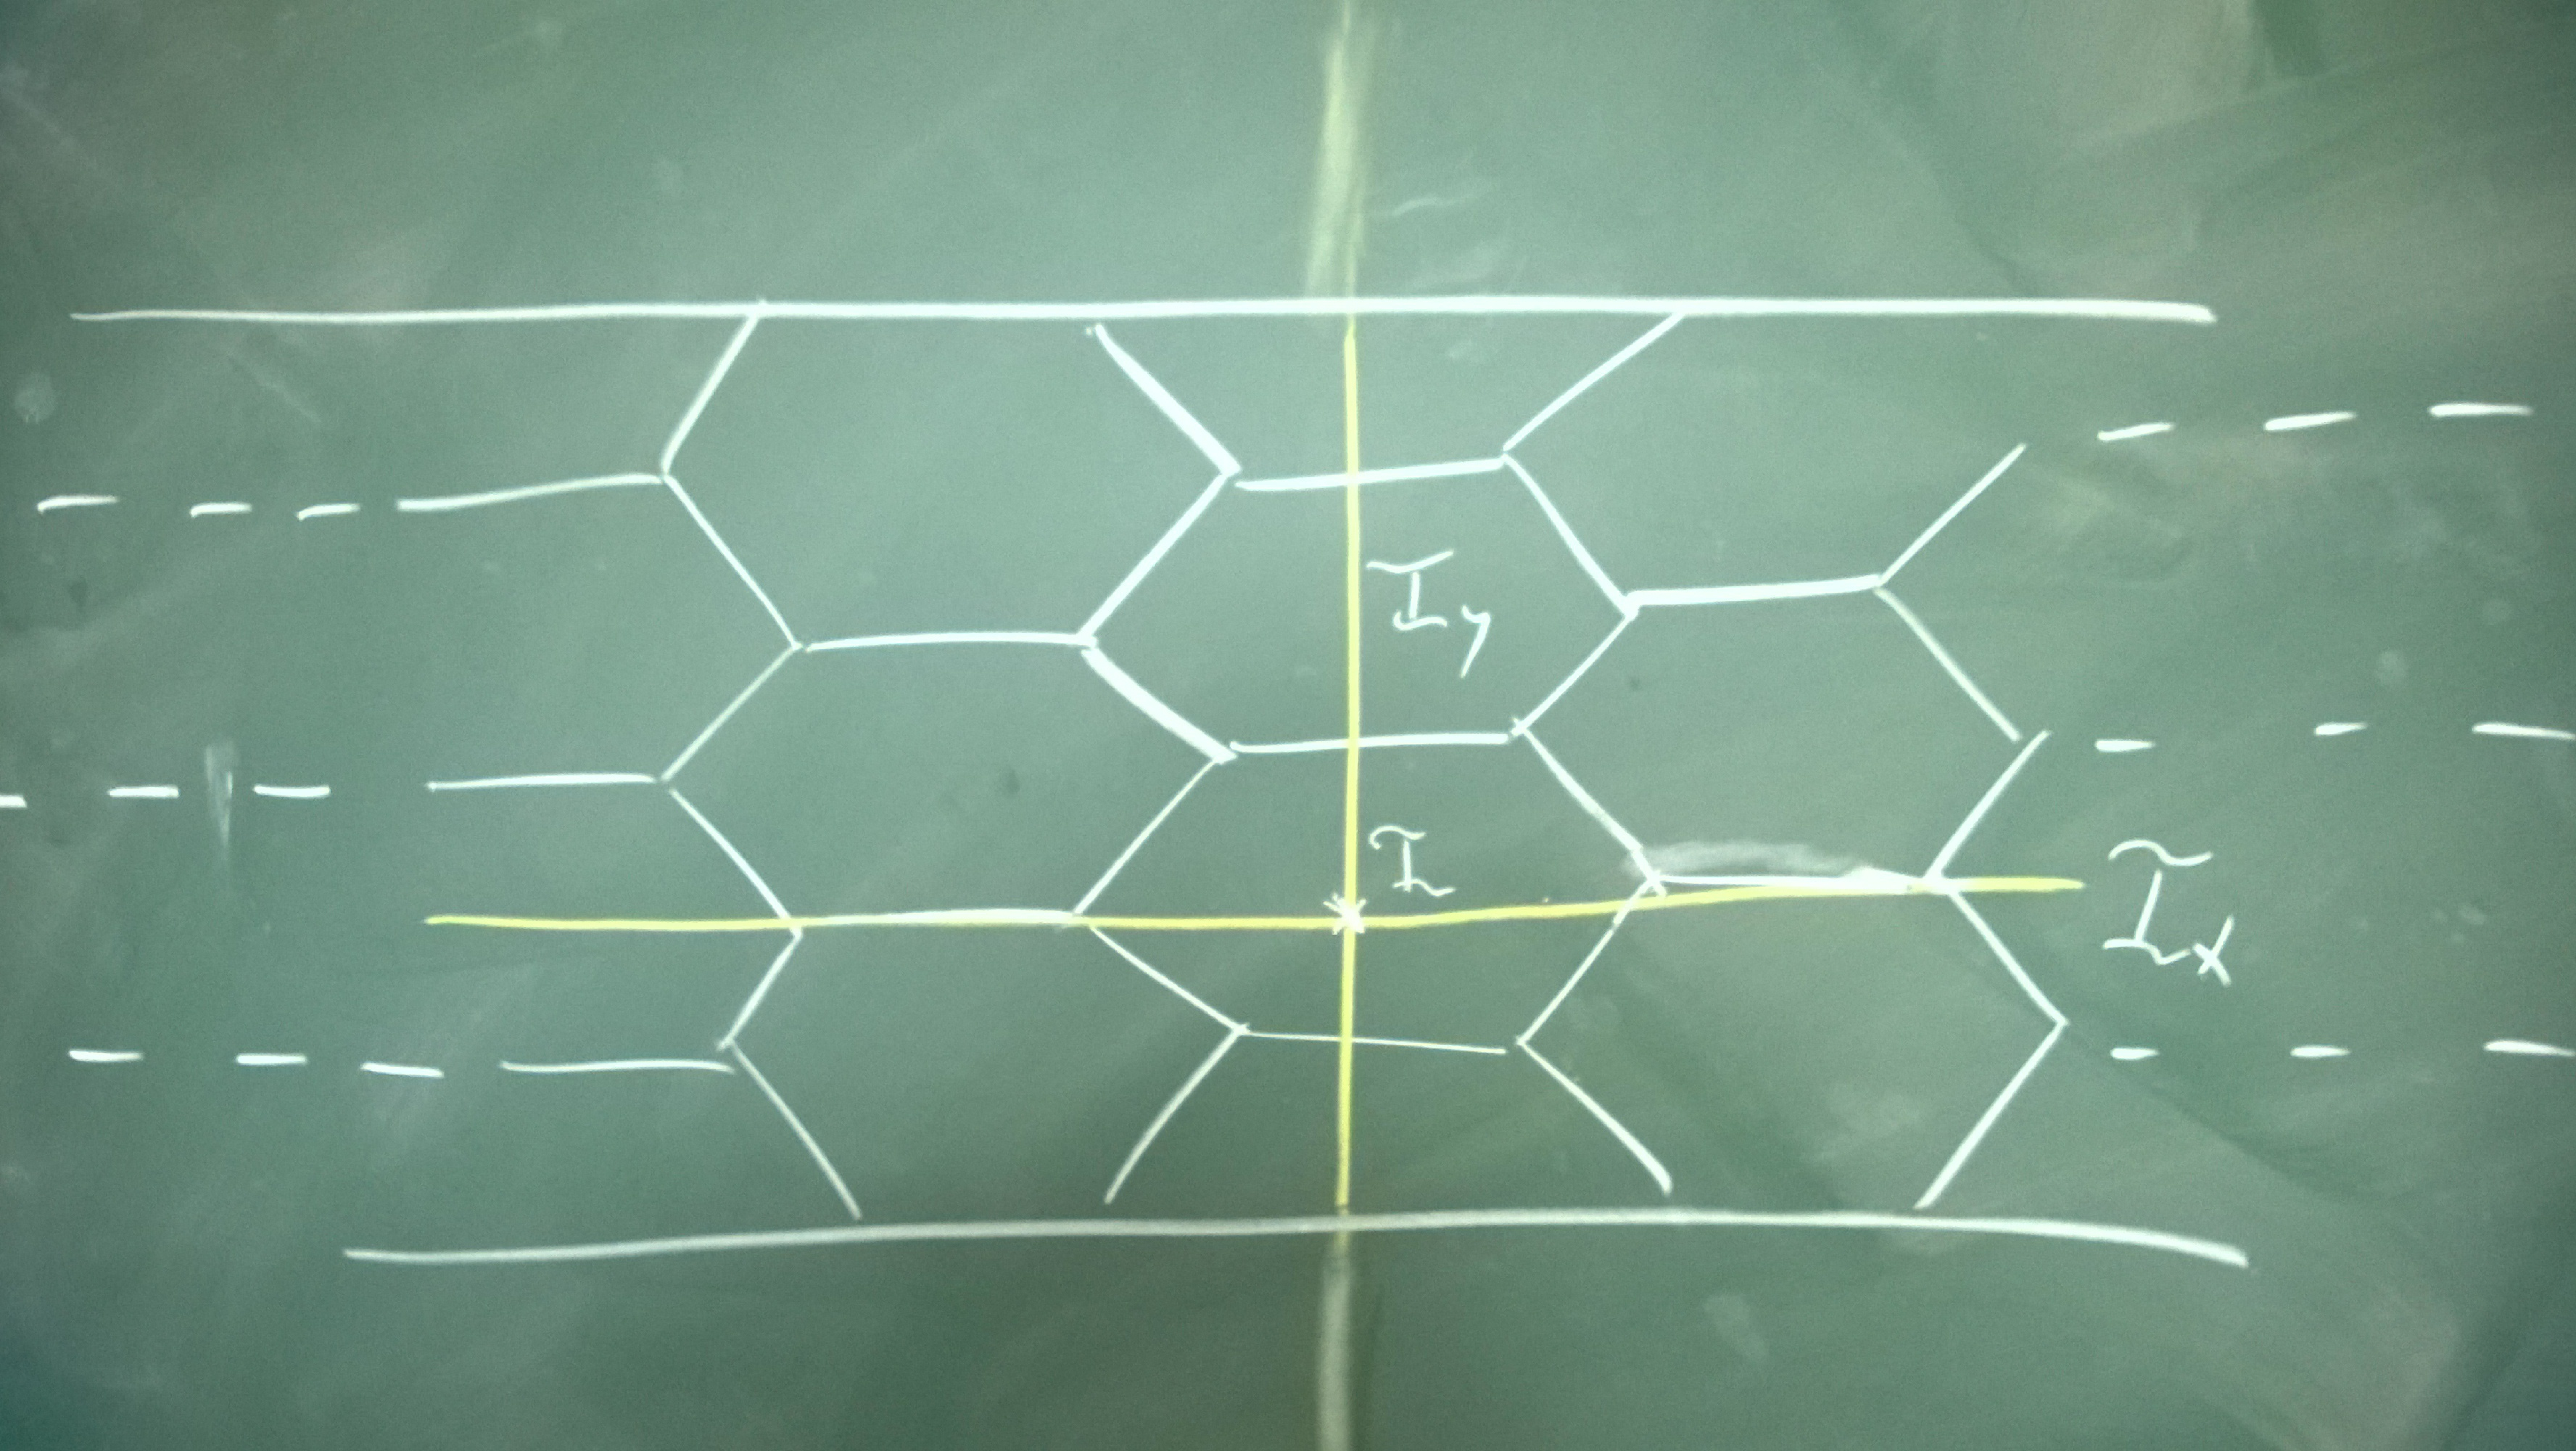
\includegraphics[width=0.8\columnwidth]{../images/symmetries.pdf}
  \caption{Lattice symmetries considered here:
  (i) $\I_x$ reflection about a line parallel to the long direction of the cylinder,
  (ii) $\I_y$ reflection about a line perpendicular to the long direction, corresponding to the entanglement
  cut shown in Fig.~\ref{fig:FBI_PEPS_2}. These are both chosen such that the reflection line
  crosses the hexagon center. Their product, $\I = \I_x \I_y$, thus represents (iii) the inversion about
  a hexagon center. \label{fig:symm} }
\end{figure}

By choosing a cylinder geometry, we explicitly break some of the lattice rotational
and reflection symmetries. The remaining symmetries are generated by
translations $T_x$ parallel and $T_y$ perpendicular to the cylinder axis
as well as reflections $\I_x$ about a line parallel and $\I_y$ about a line perpendicular to 
the cylinder axis. We also consider lattice inversion $\I = \I_x \I_y$, equivalent to a $\pi$ 
rotation of the spatial plane about the center of a hexagonal plaquette. These symmetries are
illustrated in Fig.~\ref{fig:symm}.
We find that a number of symmetry-protected topological invariants that are defined through these symmetries
take non-trivial values in the HFBI, thus protecting the doubly degenerate entanglement spectrum
on odd circumference cylinders. The complete list of non-trivial invariants is summarized in
Table~\ref{table:sym}. 

The crucial ingredient underlying these SPT invariants is a spatial symmetry $h$ that swaps the 
two sides of the entanglement cut. 
By a general symmetry analysis of \eqnref{eq:isymschmidt2}, $V_h$ must act as a 
particle-hole symmetry on the edge, since the Schmidt pairing $S$ (\eqnref{eq:S}) pairs states with
opposite quantum numbers. In this case, the symmetry action $V_{\I_y}$ is precisely
that of a particle-hole transformation in the local PEPS basis; defining $\vket{\vec{\sigma}}=\vket{\sigma_1,\ldots,\sigma_W}$
and $\vket{1-\vec{\sigma}}=\vket{1-\sigma_1,\ldots,1-\sigma_W}$, we find
\begin{equation}
V_{\I_y}\vket{\vec{\sigma}} = \vket{1-\vec{\sigma}}
\end{equation}
since a state where the $i^{th}$ hexagon contributes $\sigma_i$ bosons on the right is paired with
a state where the $i^{th}$ hexagon contributes $1-\sigma_i$ on the left. We can thus read off
that $V_{\I_y}$ acts like $\sigma_x$ in the space spanned by the states
$\lbrace \vket{\vec{\sigma}}, \vket{1-\vec{\sigma}} \rbrace$.

When $W$ is odd, these states have opposite charge parity. Specifically, if $\varPi = e^{i \pi \mathcal{Q}} \in U(1)$
is the charge parity symmetry, we have
\begin{align}
V_{\varPi} \vket{\vec{\sigma}} &= (-1)^{\sum \sigma_i} \vket{\vec{\sigma}} \\
V_{\varPi} \vket{1-\vec{\sigma}} &= (-1)^{\sum (1-\sigma_i) } \vket{1-\vec{\sigma}} \\ &= (-1)^W (-1)^{\sum \sigma_i} \vket{1-\vec{\sigma}}
\end{align}
Therefore, for $W$ odd, $V_{\varPi}$ acts like $\sigma_z$ in the space $\lbrace \vket{\vec{\sigma}}, \vket{1-\vec{\sigma}} \rbrace$.
It is thus reasonable to expect that the combination of these two symmetries acts as $V_{\varPi \I} = \sigma_x \sigma_z$,
which would obey the property that $V_{\varPi \I} V_{\varPi \I}^* = -I$ and thus form a topological invariant.

\begin{table}
\begin{tabular*}{\columnwidth}{@{\extracolsep{\stretch{1}}}*{5}{r}@{}}
\toprule
Group & Generators & Invariant & $i$ &$e, k$ \\
\midrule
$\mathbb{Z}_2^P$ & $\{\varPi \I \}$ 
& $V_{\varPi \I} V_{\varPi \I}^* = -I$ &$-$ & $ -, +$  \\
$\mathbb{Z}_2^P$ & $\{\varPi \I_y \}$ 
&$V_{\varPi \I_y} V_{\varPi \I_y}^* = -I$ &$-$ & $ -, -$\\ \hline
$\mathbb{Z}_2 \times \mathbb{Z}_2^{PT}$& $\{\varPi, \tau \I\}$ 
&$V_{\varPi} V_{\tau \I} V_{\varPi}^{-1} V_{\tau \I}^{-1} = -I$ &$+$ & $ -, -$\\
$\mathbb{Z}_2 \times \mathbb{Z}_2^{PT}$& $\{\varPi, \tau \I_y\}$
&$V_{\varPi} V_{\tau \I_y} V_{\varPi}^{-1} V_{\tau \I_y}^{-1} = -I$ &$+$ & $ -, +$\\
$\mathbb{Z}_2 \times \mathbb{Z}_2^{PT}$& $\{\varPi \I_x, \tau \I\}$
&$V_{\varPi \I_x} V_{\tau \I} V_{\varPi \I_x}^{-1} V_{\tau \I}^{-1} = -I$ &$+$ & $ -, ?$\\
$\mathbb{Z}_2 \times \mathbb{Z}_2^{PT}$& $\{\varPi \I_x, \tau \I_y\}$
&$V_{\varPi \I_x} V_{\tau \I_y} V_{\varPi \I_x}^{-1} V_{\tau \I_y}^{-1} = -I$ &$+$ & $ -, ?$\\
\bottomrule
\end{tabular*}
\caption{Summary of symmetry protecting invariants found for the HFBI state. 
The degenerate entanglement spectrum cannot be split unless all 6 of the  minimal protecting symmetry groups are broken.
\bela{What do the last three columns mean?}}
\label{table:sym}
\end{table}

We can independently calculate this numerically by performing an explicit calculation in the
canonical form of an MPS representation of the state, as outlined in Appendix~\ref{Appendix:MPS}.
We thus confirm SPT invariants for symmetries that involve such a spatial symmetry $h$ and
an on-site symmetry.
There are several appropriate invariants, as listed in Table.~\ref{table:sym}; the simplest is
\begin{equation}
V_{\varPi \I} V_{\varPi \I}^* = -I. 
\end{equation}
From this we see that the charge, translation, and inversion symmetry can all 
be broken without splitting the entanglement degeneracy, as long as the single combined symmetry
$\varPi \I $ is preserved. In Section~\ref{sec:perturbations}, we will discuss perturbations that preserve
this symmetry.

We note that there are also symmetries that act unitarily on the edge and yield SPT invariants;
however, these must form the group $\mathbb{Z}_2 \times \mathbb{Z}_2$ as $\mathbb{Z}_2$
does not have unitary projective representations. Examples for this are formed by involving
time-reversal symmetry; since $V_{\tau}$ and $V_{\I}$ both act antiunitarily, $V_{\tau \I}$ acts
unitarily on the edge. The $\mathbb{Z}_2 \times \mathbb{Z}_2$ group generated by
$\tau \I$ and $\varPi$ has a projective representation characterized by the 
topological invariant
\beq
V_{\varPi} V_{\tau \I} V_{\varPi}^{-1} V_{\tau \I}^{-1}
 = - I.
\eeq
This symmetry protection gives a distinct class of perturbations that cannot
split the entanglement degeneracy.
%For the HFBI state itself, $V_{\tau}$ acts as the identity in 
%the basis $\vket{\{\sigma_i\}}$, so this equation follows trivially from 
%Equation~\ref{eq:hfbisym}. 
The complete set of symmetry groups we find is summarized in Table~\ref{table:sym}.

We can form variants of the HFBI state, which are unitarily related to the original
state by an on-site unitary and thus share the same entanglement spectrum, where
the entanglement degeneracy can be protected by a lattice symmetry alone without involving
the on-site $\varPi$ symmetry. These will be discused further in Appendix~\ref{Appendix:Variants}.

%It is easy to produce a variant on the HFBI state - unitarily related to the original
%state by an on-site unitary and thus with the same entanglement spectrum - where the role
%of $\varPi \I$ is played by $\I$. The degeneracy in this state would be unsplit by a uniform
%field instead of a staggered field, which may be physically more interesting. 
%This is discussed further in Appendix~\ref{Appendix:Variants}.
